%%%%%%%%%%%%%%%%%%%%%%%%%%%%%%%%%%%%%%%%%%%%%%%%%%%%%%%%%%%%%%%%%%%%%%%%%%%%%%%%%%%%%%%%%%%%%%%%%%%%%%%%%%%%%%%%%%%%%%%%%%%%%%%%%%%%%%%%%%%%%%%%%%%%%%%%%%%%%%%%%%%%%%%
%%%%%%%%%%%%%%%%%%%%%%%%%%%%%%%%%%%%%%%%%%%%%%%%%%%%%%%%%%%%%%%%%%%%%%%%%%%%%%%%%%%%%%%%%%%%%%%%%%%%%%%%%%%%%%%%%%%%%%%%%%%%%%%%%%%%%%%%%%%%%%%%%%%%%%%%%%%%%%%%%%%%%%%
%%%%%%%%%%%%%%%%%%%%%%%%%%%%%%%%%%%%%%%%%%%%%%%%%%%%%%%%%%%%%%%%%%%%%%%%%%%%%%%%%%%%%%%%%%%%%%%%%%%%%%%%%%%%%%%%%%%%%%%%%%%%%%%%%%%%%%%%%%%%%%%%%%%%%%%%%%%%%%%%%%%%%%%
%%%%%%%%%%%%%%%%%%%%%%%%%%%%%%%%%%%%%%%%%%%%%%%%%%%%%%%%%%%%%%%%%%%%%%%%%%%%%%%%%%%%%%%%%%%%%%%%%%%%%%%%%%%%%%%%%%%%%%%%%%%%%%%%%%%%%%%%%%%%%%%%%%%%%%%%%%%%%%%%%%%%%%%

\FloatBarrier
\chapter{Results}
\label{sec:Results}

After developing the methods of the background estimation for all different background sources and their corresponding systematic uncertainties (all explained in Section~\ref{ch:BackgroundEstimation}), 
the search is performed in four exclusive signal regions with 19.7\fbinv of data collected at a centre-of-mass energy of $\sqrt{s} = 8\tev$ at the CMS experiment.
The predicted numbers of events for the fake and the leptonic background in the four signal regions are listed in Table~\ref{tab:BackgroundPrediction}.
It can be seen, that fake tracks are by far the dominant background to this search.
The leptonic background contributes only in one signal region to the total background with a share of about 10\%.

%\renewcommand{\arraystretch}{1.5}
%\begin{table}[!t]
%\centering
%\caption{Background prediction in the four exclusive signal regions for the fake and the leptonic background.}
%\label{tab:BackgroundPrediction}
%\makebox[0.99\textwidth]{
%\begin{tabular}{c |c| c }
%\multicolumn{3}{c}{} \\
%\toprule
%Signal region                                & Fake Bkg                                             & Leptonic Bkg  \\
%\midrule
%$\pt: 30-50\gev$ / $\ias:0.05-0.30$          & 19.11 $^{+ 2.61} _{- 2.61}$ (stat) $\pm$ 9.35 (sys)      & 0.00 $^{+ 2.58} _{- 0.00}$ (stat) $\pm$ 0.00 (sys) \\
%$\pt: 50-\infty\gev$ / $\ias:0.05-0.30$      & 22.21 $^{+ 3.60} _{- 3.60}$ (stat) $\pm$ 8.78 (sys)      & 2.17 $^{+ 2.99} _{- 1.34}$ (stat) $\pm$ 1.65 (sys) \\
%$\pt: 30-50\gev$ / $\ias:0.30-1.00$          & 2.49 $^{+ 0.85} _{- 0.85}$ (stat) $\pm$ 1.98 (sys)       & 0.00 $^{+ 0.22} _{- 0.00}$ (stat) $\pm$ 0.00 (sys) \\
%$\pt: 50-\infty\gev$ / $\ias:0.30-1.00$      & 2.52 $^{+ 1.14} _{- 1.14}$ (stat) $\pm$ 1.27 (sys)       & 0.04 $^{+ 0.30} _{- 0.03}$ (stat) $\pm$ 0.03 (sys) \\
%\bottomrule
%\multicolumn{3}{c}{}\\
%\end{tabular}}
%\end{table}

\renewcommand{\arraystretch}{2.0}
\begin{table}[!h]
\centering
\caption{Background prediction in the four exclusive signal regions for the fake and the leptonic background.}
\label{tab:BackgroundPrediction}
\makebox[0.99\textwidth]{
\begin{tabular}{c| c| c | c }
\multicolumn{4}{c}{} \\
\toprule
\multicolumn{2}{c|}{Signal region}                                & Fake Bkg                                             & Leptonic Bkg  \\
\multicolumn{1}{c}{\pt}   & \ias & & \\ 
\midrule
30-50\gev       &0.05-0.30      & 19.11 $^{+ 2.61} _{- 2.61}$ (stat) $\pm$ 9.35 (sys)      & 0.00 $^{+ 2.58} _{- 0.00}$ (stat) $\pm$ 0.00 (sys) \\
50-$\infty$\gev   &0.05-0.30      & 22.21 $^{+ 3.60} _{- 3.60}$ (stat) $\pm$ 8.78 (sys)      & 2.17 $^{+ 2.99} _{- 1.34}$ (stat) $\pm$ 1.65 (sys) \\
30-50\gev       &0.30-1.00      & 2.49 $^{+ 0.85} _{- 0.85}$ (stat) $\pm$ 1.98 (sys)       & 0.00 $^{+ 0.22} _{- 0.00}$ (stat) $\pm$ 0.00 (sys) \\
50-$\infty$\gev   &0.30-1.00      & 2.52 $^{+ 1.14} _{- 1.14}$ (stat) $\pm$ 1.27 (sys)       & 0.04 $^{+ 0.30} _{- 0.03}$ (stat) $\pm$ 0.03 (sys) \\
\bottomrule
\multicolumn{4}{c}{}\\
\end{tabular}}
\end{table}

Finally, the comparison between the predicted number of events and the number of observed events is shown in Fig.~\ref{fig:FinalResult}.
The results are compatible with the Standard Model background within 1$\sigma$ uncertainties in all four signal regions.
No excess above the SM prediction is observed in either of the four signal regions.
Thus, no evidence for physics beyond the Standard Model could be found.

Therefore, in the following section these results will be used to constrain the parameter space of supersymmetric models with almost mass degenerate charginos and neutralinos.

\begin{figure}[!b]
  \centering 
  \begin{tabular}{c}
    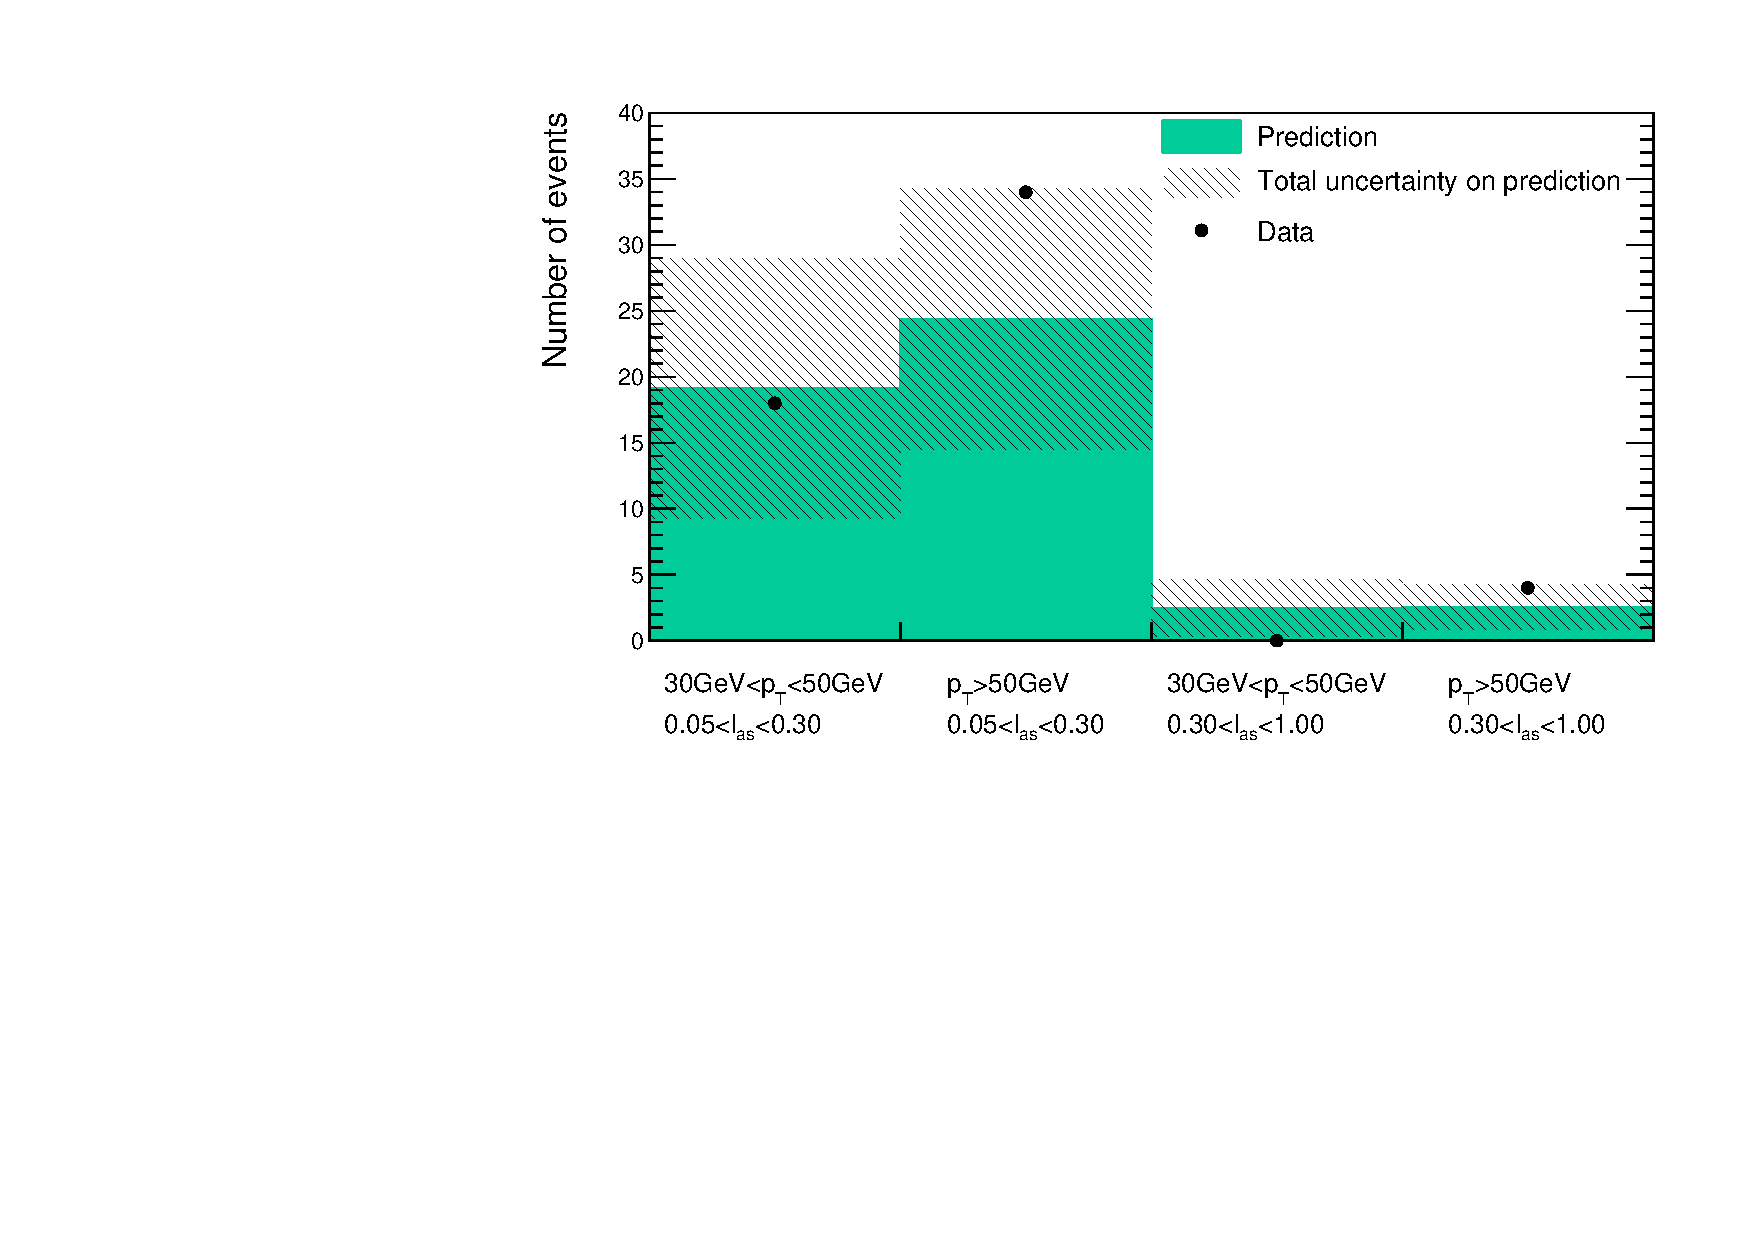
\includegraphics[width=0.98\textwidth]{figures/analysis/Results/FinalResultPlot.pdf} 
  \end{tabular}
  \caption{Number of predicted (green area) and observed (black dots) events for the four different signal regions. The hashed area represents the total uncertainty on the background prediction.}
  \label{fig:FinalResult}
\end{figure} 
Additionally, the corresponding numbers of predicted and observed events can be found in Table~\ref{tab:FinalResult}.
%\renewcommand{\arraystretch}{1.5}
%\begin{table}[!t]
%\centering
%\caption{Number of predicted and observed events for the four different signal regions.}
%\label{tab:FinalResult}
%\makebox[0.99\textwidth]{
%\begin{tabular}{l |c| c}
%\multicolumn{3}{c}{} \\
%\toprule
%Signal region                         & Prediction                                              & Observation  \\
%\midrule
%$\pt: 30-50\gev$ / $\ias:0.05-0.30$      & 19.11 $^{+ 3.67} _{- 2.61}$ (stat) $\pm$ 9.35 (sys)         & 18           \\
%$\pt: 50-\infty\gev$ / $\ias:0.05-0.30$  & 24.38 $^{+ 4.68} _{- 3.84}$ (stat) $\pm$ 8.93 (sys)         & 34           \\
%$\pt: 30-50\gev$ / $\ias:0.30-1.00$     & 2.49 $^{+ 0.87} _{- 0.85}$ (stat) $\pm$ 1.98 (sys)          & 0            \\
%$\pt: 50-\infty\gev$ / $\ias:0.30-1.00$ & 2.57 $^{+ 1.18} _{- 1.14}$ (stat) $\pm$ 1.27 (sys)          & 4            \\
%\bottomrule
%\multicolumn{3}{c}{} \\
%\end{tabular}}
%\end{table}


\renewcommand{\arraystretch}{2.0}
\begin{table}[!t]
\centering
\caption{Number of predicted and observed events for the four different signal regions.}
\label{tab:FinalResult}
\makebox[0.99\textwidth]{
\begin{tabular}{c |c |c| c}
\multicolumn{4}{c}{} \\
\toprule
\multicolumn{2}{c|}{Signal region}                                & Fake Bkg                                             & Leptonic Bkg  \\
\multicolumn{1}{c}{\pt}   & \ias & & \\ 
\midrule
30-50\gev       & 0.05-0.30  & 19.11 $^{+ 3.67} _{- 2.61}$ (stat) $\pm$ 9.35 (sys)         & 18           \\
50-$\infty$\gev & 0.05-0.30  & 24.38 $^{+ 4.68} _{- 3.84}$ (stat) $\pm$ 8.93 (sys)         & 34           \\
30-50\gev       & 0.30-1.00  & 2.49 $^{+ 0.87} _{- 0.85}$ (stat) $\pm$ 1.98 (sys)          & 0            \\
50-$\infty$\gev & 0.30-1.00  & 2.57 $^{+ 1.18} _{- 1.14}$ (stat) $\pm$ 1.27 (sys)          & 4            \\
\bottomrule
\multicolumn{4}{c}{} \\
\end{tabular}}
\end{table}

%\renewcommand{\arraystretch}{1.5}
%\begin{table}[!h]
%\centering
%\caption{Background prediction from the four different background sources: Fakes, taus, muons and electrons.}
%\label{tab:FinalResult}
%\makebox[0.99\textwidth]{
%\begin{tabular}{l |c| c | c| c}
%\multicolumn{3}{c}{} \\
%\toprule
%Signal region                         & Fakes   & Taus  & Muons & Electrons  \\
%\midrule
%$30\gev<\pt<50\gev$ / $0.05<\ias<0.3$ & 19.11 $^{+ 2.61} _{- 2.61}$ (stat) $\pm$ 9.35 (sys)      & 0.00 $^{+ 0.87} _{- 0.00}$ (stat) $\pm$ 0.00 (sys) & 0.00 $^{+ 0.22} _{- 0.00}$ (stat) $\pm$ 0.00 (sys) & 0.00 $^{+ 2.42} _{- 0.00}$ (stat) $\pm$ 0.00 (sys)                           \\
%$\pt>50\gev$        / $0.05<\ias<0.3$ & 22.21 $^{+ 3.60} _{- 3.60}$ (stat) $\pm$ 8.78 (sys)      & 0.00 $^{+ 0.33} _{- 0.00}$ (stat) $\pm$ 0.00 (sys) & 0.00 $^{+ 0.29} _{- 0.00}$ (stat) $\pm$ 0.00 (sys) & 2.17 $^{+ 2.96} _{- 1.34}$ (stat) $\pm$ 1.65 (sys)                             \\
%$30\gev<\pt<50\gev$ / $\ias>0.3$      & 2.49 $^{+ 0.85} _{- 0.85}$ (stat) $\pm$ 1.98 (sys)       & 0.00 $^{+ 0.01} _{- 0.00}$ (stat) $\pm$ 0.00 (sys) & 0.00 $^{+ 0.22} _{- 0.00}$ (stat) $\pm$ 0.00 (sys) & 0.00 $^{+ 0.05} _{- 0.00}$ (stat) $\pm$ 0.00 (sys)                      \\
%$\pt>50\gev$        / $\ias>0.3$      & 2.52 $^{+ 1.14} _{- 1.14}$ (stat) $\pm$ 1.27 (sys)       & 0.00 $^{+ 0.00} _{- 0.00}$ (stat) $\pm$ 0.00 (sys) & 0.00 $^{+ 0.29} _{- 0.00}$ (stat) $\pm$ 0.00 (sys) & 0.04 $^{+ 0.06} _{- 0.03}$ (stat) $\pm$ 0.03 (sys)                      \\
%\bottomrule
%\multicolumn{3}{c}{} \\
%\end{tabular}}
%\end{table}


%%%%%%%%%%%%%%%%%%%%%%%%%%%%%%%%%%%%%%%%%%%%%%%%%%%%%%%%%%%%%%%%%%%%%%%%%%%%%%%%%%%%%%%%%%%%%%%%%%%%%%%%%%%%%%%%%%%%%%%%%%%%%%%%%%%%%%%%%%%%%%%%%%%%%%%%%%%%%%%%%%%%%%%
%%%%%%%%%%%%%%%%%%%%%%%%%%%%%%%%%%%%%%%%%%%%%%%%%%%%%%%%%%%%%%%%%%%%%%%%%%%%%%%%%%%%%%%%%%%%%%%%%%%%%%%%%%%%%%%%%%%%%%%%%%%%%%%%%%%%%%%%%%%%%%%%%%%%%%%%%%%%%%%%%%%%%%%

